\documentclass[12pt]{article}
\usepackage{geometry}

%\usepackage[margin=0.2in]{geometry}                
\geometry{letterpaper}                  
\usepackage{graphicx}
\usepackage{tipa}
\usepackage{upgreek}
\usepackage{amsmath, amssymb, amsthm}
\newtheorem{theorem}{Theorem}
\newtheorem{corollary}{Corollary}
\newtheorem{proposition}{Proposition}
\newtheorem{lemma}{Lemma}
\newtheorem{definition}{Definition}
\newtheorem{remark}{Remark}
\newtheorem{notation}{Notation}
\newcommand{\N}{\mathcal{N}}
\newcommand{\Bern}{\textrm{Bern}}
\newcommand{\Bin}{\textrm{Bin}}
\newcommand{\Beta}{\textrm{Beta}}
\newcommand{\Gam}{\textrm{Gamma}}
\newcommand{\Expo}{\textrm{Expo}}
\newcommand{\Pois}{\textrm{Pois}}
\newcommand{\Geom}{\textrm{Geom}}
\begin{document}


\begin{center} \textbf{Programming Assignment 2} \end{center}
 \vspace{-7mm} 
\begin{flushright} Lexi Ross \& Julia Winn  \end{flushright}

 \vspace{-4mm} 
\noindent \textbf{Part 1 Writeup}
\medskip

\noindent If all arithmetic operations (adding, subtracting, multiplying or dividing two real numbers) is cost 1, then we can calculate the recurrence for Strassen's algorithm by computing the base case, and all powers of $n$ that follow.
\medskip

\noindent Consider a $2 \times 2$ matrix.  It's costs using Strassen's algorithm and normal matrix multiplication can be calculated as follows:

\begin{itemize}
\item $P_1, P_2, P_3, P_4$ cost 2 each
\item $P_5, P_6, P_7$ cost 3 each
\item $AE + BG$ and $CF + DH$ cost 3 each
\item $AF + BH$ and $CE + DG$ cost 1 each
\end{itemize}

\noindent T(1) = 1
\medskip

\noindent T(2) = $(2 \times 4) + (3 \times 3) + (3 \times 2) + (1 \times 2)= 8 + 9 + 6 + 2 = 25$
\medskip

\noindent T(4) =  247
\medskip

\noindent T(n) = $4((\frac{n}{2})^2 + T(\frac{n}{2})) + 3(2(\frac{n}{2})^2 + T(\frac{n}{2})) + 8(\frac{n}{2})^2$
\bigskip

\noindent Our recurrence relation for Strassen's algorithm is $T(n) = 18(\frac{n}{2})^2 + 7\cdot T(\frac{n}{2})$ where $n=2^x, n >1$
\bigskip

\noindent Using Mathematica we can solve for the recurrence relation to find:

$$T(n) = 7^{\frac{\log(2n)}{\log(2)}} - 6n^2$$

\noindent However we don't actually want the recurrence relation because this will not take into account the crossover point.  Any value of $n$ we plug in will only return the total cost if we were \emph{only} using Strassen's algorithm, which will be much higher than a combination where we eventually switch to normal matrix multiplication.
\bigskip

\noindent However, because our normal matrix multiplication will go all the way down to the base case of 1, we \emph{do} want to solve the recurrence relation for regular matrix multiplication.  
\medskip

\noindent One "even conventional" algorithm for multiplying matrices is the sum over the rows and columns where 
$$c_{i,k} = \sum_k a_{ij} \cdot b_{jk}$$

\noindent The complexity is roughly $2n^3$ but more specifically $n^2(2n-1)$ because every item takes $n$ multiplications and $n-1$ sums.  You can also find this by solving for the recurrence relation $T(n) = n^2 + 8T(\frac{n}{2}) \to T(n) = n^2(2n-1)$
\bigskip

\noindent Now our goal is to either find the lowest value of n such that using Strassen's algorithm will yield a greater value than just using conventional matrix multiplication or the highest value where using 
\medskip

\noindent We want to solve for:

$$n^2(2n-1) \approx 7 \cdot \bigg( \frac{n}{2}\bigg)^2\bigg(2\frac{n}{2}-1\bigg) + 18\bigg( \frac{n}{2}\bigg)^2$$

$$n^2(2n-1) \approx \frac{7}{4}(n-1)n^2 + \frac{9n^2}{2}$$

\smallskip
\noindent Plugging this into Wolfram Alpha we find $n\approx15$, so theoretically it is optimal to use Strassen's algorithm at the crossover point of $\approx$ 15 and greater.  However because to use Strassen's algorithm any number that is not a power of 2 will need to eventually be padded so that it becomes one, so all numbers greater than 8 and less than 16 will be padded with zeros until they are 16 by 16 matrices.

%lowest strassens greater, highest strassen's less
\bigskip

\noindent \textbf{Experimental Analysis}
\bigskip

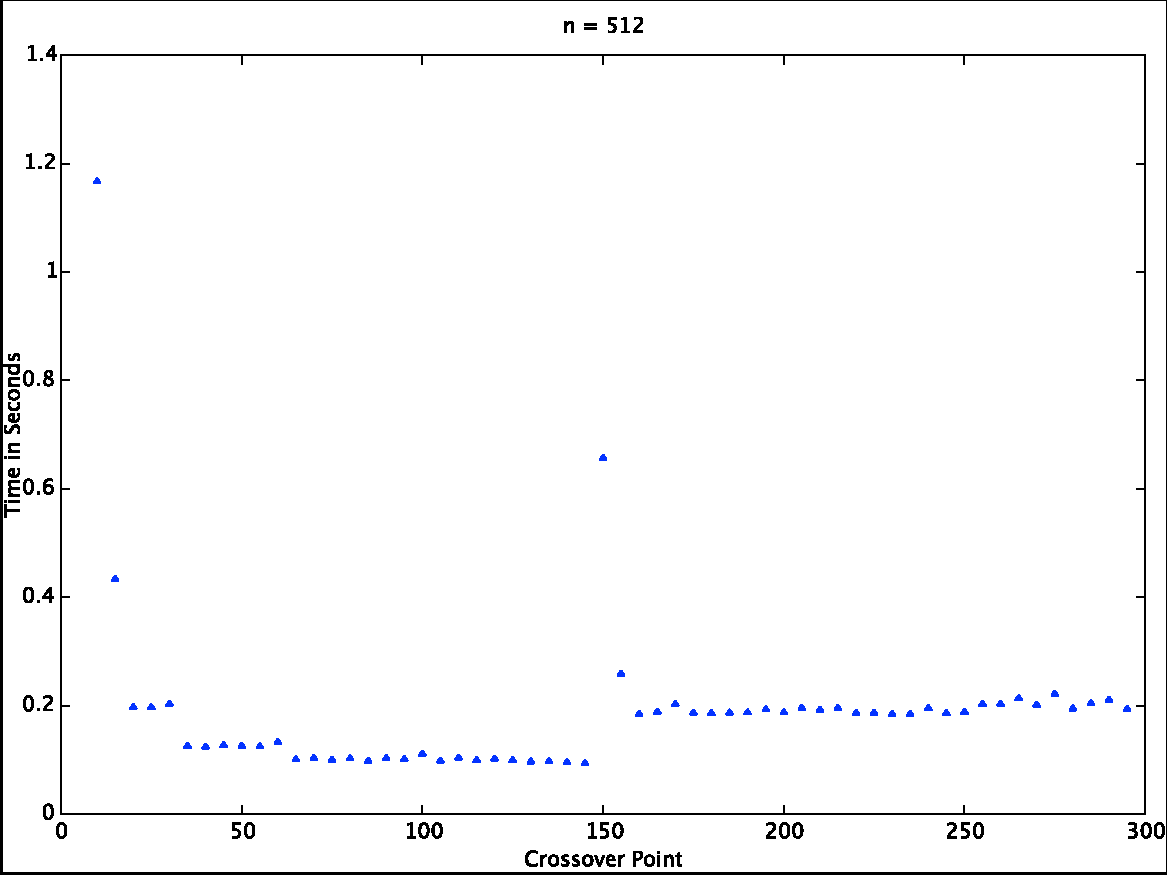
\includegraphics[scale=0.6]{512.pdf}

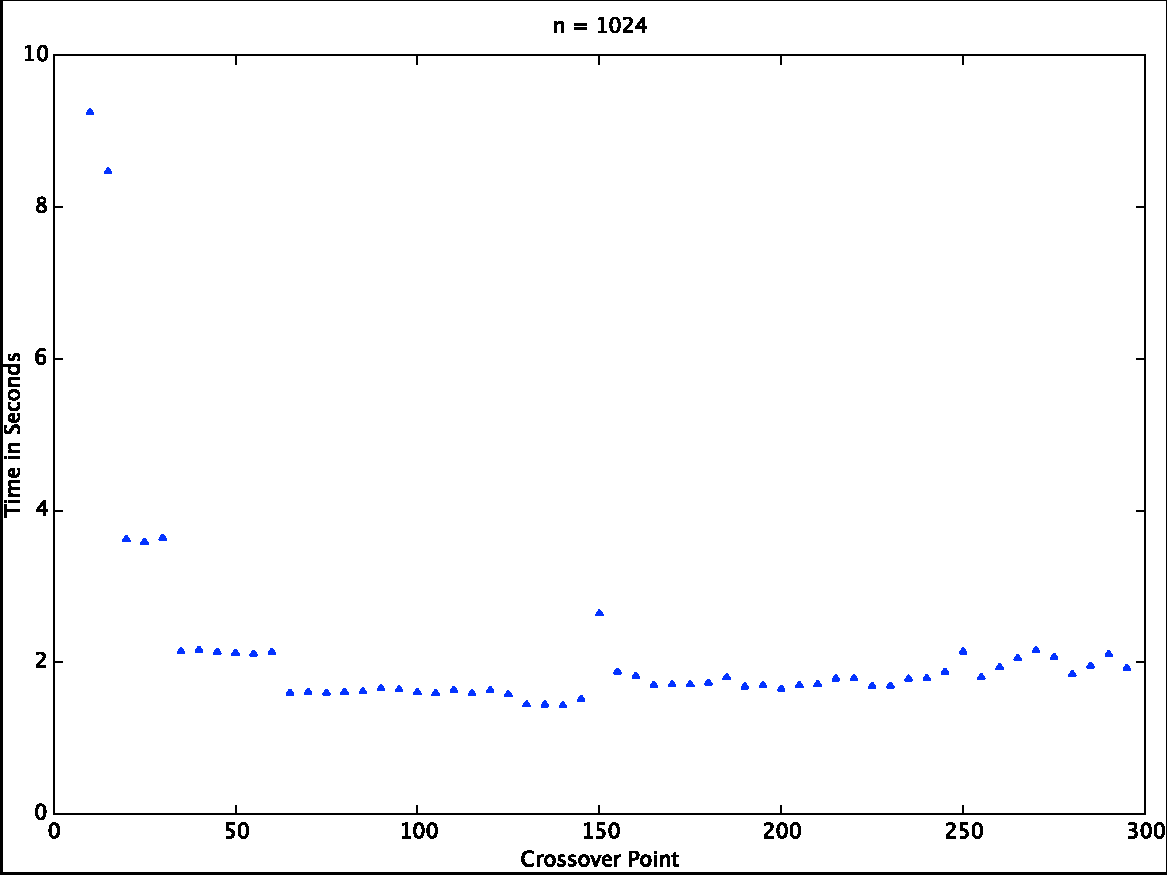
\includegraphics[scale=0.6]{1024.pdf}

\includegraphics[scale=0.6]{2048.pdf}

\noindent \textbf{Optimizations}
\bigskip

\noindent Coding in Java, we started off with a naive implementation. We decided to represent matrices using a thin wrapper class around two-dimensional integer arrays. We coded the conventional algorithm naively (see below), and for Strassen's algorithm, we simply followed the algorithm from the lecture notes, allocating new matrices for each of the 8 submatrices as well as each of the 7 products. However, after testing our code with large values, we realized that the algorithm was running quite slowly (up to 8 seconds for large values of n). We then made the following optimizations to our code:
\medskip

\noindent To improve the caching performance of the conventional algorithm, we noted that an ideal method would access all elements of each row before moving onto the next row, taking advantage of cache localization. However, the native implementation involves cycling through the rows of one matrix and the columns of another. We fixed this inefficiency by switching the order of the nested loops, which has the effect of cycling through the rows of both matrices, slowly building up each final entry by using k (the traditional inner loop) as the outermost loop. Rather than constructing each final dot product in a series of subsequent operations, we gradually build each dot product while obeying the natural iteration order (as dictated by hardware).
\bigskip

\noindent Next, we set out to improve the space performance of Strassen's algorithm. Instead of allocating new heap space for the submatrices, as we did initially, we allowed the two original matrices as data storage throughout the course of the algorithm, and simply mutated (and then reverted) certain parts of these two matrices. Instead of passing around smaller and smaller matrices to multiply into the function, as might be typical of a recursive pattern, we pass in the two original matrices to each recursive call, along with several other variables that determine the left and top bounds of each matrix to multiply as well as the size of these matrices (working with square matrices allowed us to cut some corners and pass fewer arguments). For example, we need to obtain the first product, p1, by multiplying A(F-H). We are given top1, left1, top2, and left2, which represent the top and left bounds of the outer matrices we are multiplying; we can think of these as offsets. In order to find p1, we first look at the upper right fourth of m2 (offset by top2 and left2) (F) and subtract each entry by the equivalent entry in the bottom right fourth (H). We then recursively call the Strassen algorithm, passing in top1 and left1 (those don't change since A is situated at the upper left corner), and top2 and (left2+half), where half=n/2. Once this recursive call returns a matrix (p1), we add the entries of p1 to the appropriate corner(s) of the return matrix (in this case, upper right and lower right). Finally, we then add the entries of H back into F, as a way of resetting before finding the next product. Note that we also save space by writing the results of the recursive call directly into what will become the return matrix. This way, we are free to overwrite p1 with the next product!
\bigskip

\noindent While it seems that this space-saving technique would cost us time because of all the iterations, it ended up running just as fast if not faster than our naive implementation. We suspect that this is because memory allocation actually takes up more time than iterating through a two-dimensional array. Before the improvement, in each level of recursion, we were allocating space for 19 matrices of size n/2 and 1 matrix of size n (the return value). Now, we allocate space for just 1 matrix of size n/2 (to store the products) and 1 matrix of size n (to store what will eventually be returned). While not asympotically significant, this is a very significant constant factor difference, particularly when dealing with very large matrices!

\bigskip

\noindent \textbf{Padding}
\bigskip

\noindent As our implementation must work even when $n$ is odd, our algorithm first checked whether the size of a matrix was a power of 2, and if it was not, it calculated the next highest power of 2 after the value $n$.  
\medskip

\noindent When comparing the running times of Strassen's algorithm with conventional matrix multiplication an important factor to consider is the necessary padding when running Strassen's algorithm on values of $n$ that are not powers of 2.  This can be dealt with using padding, as long as the current $n$ is even, we can divide it into equal sub matrices, and when it is odd we must pad each matrix of this size with an additional $(2n+1)$ zeros to get an even value of $n$.
\medskip

\noindent Whether or not this process takes place at the beginning of the algorithm before the sub dividing of the matrix has begun does not change the total number of zeros added.  Therefore, regardless of the nature of the process, any matrix with a non-power of 2 $n$ will need a certain number of zeros added.  The final size of the matrix post padding is the size of the matrix we will be multiplying.
\medskip

\end{document}